\documentclass[]{article}

\usepackage[T1]{fontenc}
\usepackage{graphicx}
\usepackage{hyperref}
\usepackage{natbib}

\setlength{\parindent}{0pt} %to avoid the first line indent throughout the documen

\title{Variant calling from RNA-seq data using the GATK joint genotyping workflow}
\author{Jean-Simon Brouard}

\begin{document}

\maketitle

\begin{abstract}
Put the abstract here.
\end{abstract}

\section{Introduction}
Since the introduction of RNAseq, many researchers have seen the opportunity to use this data not only for differential expression analysis, but also for calling variants \cite{Piskol2013}. Examples of such researches include a, b, c and d. Whereas trusted bioinformatic protocols exist for detecting sequence variants on a variety of DNAseq samples (germline DNA, whole-exome sequencing etc.) that come from distinct contexts \cite{Koboldt2020}, environnemental samples), protocols designed to handle RNAseq data are scarce \cite{Piskol2013}. At present the gold-standard for variant calling on RNAseq data is the GATK Per-sample workflow although an updated detailed workflow documentation for calling variants in RNAseq data is in the roadmap of the GATK experts \cite{GATK_best_RNAseq}.


Currently, researchers interested in performing GATK variant calling on RNAseq data have the option of using the fully validated Per-sample workflow \cite{GATK_RNAseq_variant_discovery} or using an in-progress advanced workflow designed for cloud computing \cite{GATK_gatk4_rnaseq_github}.
As mentionned, the Per-sample approach has several drawbacks (cite myself)

An appealing alternative would be to follow most of the GATK Best practices relative to RNAseq data and to take advantage of joint genotyping approach which is avalaible in version 3 and 4 of GATK for germline short variants and indels (ref). The joint-genotyping method has proven to be more sensitive, more flexible and to reduce computational challenges relative to the traditional calling approach \cite{GATK_jointCalling_1}. In addition, the latter approach has the advantage to facilitate the inceremental discovery of variants that origin from distinct cohorts of samples. Technically, this can be achieved by combining parts of the GATK RNAseq workflow and parts of the GATK joint genotyping workflow.

In spite that the protocol described here largely use workflows and concepts developped by the GATK team, the reader should be aware that it has not been validated by GATK experts. We have shown previously that a similar workflow has and we did not ahve experienced any problesm (Brouard)

Here we present GATK4 and fully updated version of this approach.

an update end-to-end analysis of...



Figure 1 present the workflow proposed here.

% figure 1 





In the next section, we describe how the diverse programs required to perform the whole analysis can be installed.

\section{Materials}

\subsection{Environment}


The vast majority of commands in this tutorial have been carefully tested and fully executed on a remote linux server working with the Sun Grid Engine (SGE) workload manager. Obviously, Bash scripts presented here will need to be slightly adapted to be used with your own raw sequence data. In addition, other small changes will be required  to these scripts if another workload manager is in place on your computer cluster or if you intend to perform the analysis on a local machine.





\subsection{Installing bioinformatic programs}

\subsubsection{The GATK suite}

It is suggested to install the GATK suite in a separate conda environment. Assuming that you are familiar with the conda package management system, you could install all GATK programs in an environment called 'gatk4' with the following command:

\begin{verbatim}
conda create -n gatk4 -c bioconda gatk4 
\end{verbatim}

To generate optional plots in the Base Quality Score Recalibration subsection, additionnal libraries are required. Use the following commands to install them alongside GATK in the gatk4 environment:

\begin{verbatim}
conda activate gatk4
conda install -c conda-forge r-base
conda install -c r r-ggplot2
conda install -c r r-gplots
conda install -c bioconda r-gsalib
\end{verbatim}


\subsubsection{The NCBI SRA toolkit programs}

You can easily download public sequences from the NCBI Sequence Read Archive (SRA) using the NCBI SRA toolkit. Detailed instructions about this tool can be found at \href{https://trace.ncbi.nlm.nih.gov/Traces/sra/sra.cgi?view=toolkit_doc}{https://trace.ncbi.nlm.nih.gov/Traces/sra/sra.cgi?view=toolkit\_doc}. However, before using it, do not forget to configure the SRA toolkit program ( \href{https://github.com/ncbi/sra-tools/wiki/03.-Quick-Toolkit-Configuration}{https://github.com/ncbi/sra-tools/wiki/03.-Quick-Toolkit-Configuration}).


Once installed, export the SRA toolkit programs in you PATH:

\begin{verbatim}
export PATH=$PATH:$PWD/sratoolkit.2.10.9-ubuntu64/bin
\end{verbatim}

As usual, you can make this change persistent, by adding the previous line to your .bashrc file.


\subsubsection{The STAR aligner}

Although you can retrieve and install the STAR aligner with conda, it can be installed easily by just downloading the latest STAR source from releases:

\begin{verbatim} 
wget https://github.com/alexdobin/STAR/archive/2.7.7a.zip
unzip 2.7.7a.zip
cd STAR-2.7.7a/
\end{verbatim}

You can safely use the pre-compiled STAR executables located in the bin/ subdirectory. It is convenient to add the executables to your PATH:

\begin{verbatim}
export PATH=$PATH:$PWD/bin/Linux_x86_64
\end{verbatim}



\subsubsection{The Picard tools}

We will use the Picard tools (\href{https://broadinstitute.github.io/picard/}{https://broadinstitute.github.io/picard/}) to mark duplicated reads. One can download the pre-build java program with:

\begin{verbatim}
wget https://github.com/broadinstitute/picard/releases/download/\
2.25.0/picard.jar
\end{verbatim}

It is recommend to set up an environment variable to act as a shortcut. Again, to make it persistent in other sessions, simply, add a line to your .bashrc file:

\begin{verbatim}
export PICARD=$HOME/bioinfo_programs/picard.jar
\end{verbatim}

Then, you would be able to call Picard tools with:

\begin{verbatim}
java -jar $PICARD
\end{verbatim}


\subsubsection{Samtools, BCFtools and HTSlib}


The Samtools web site (\href{http://www.htslib.org/}{http://www.htslib.org/}) contains a plenty of informations about the Samtools suite, a collection of widely used bioinformatic programs designed to read, write, edit, index and view alignments files in the SAM, BAM and CRAM formats \cite{Danecek2021}. Less known, but just as powerful, the BCFtools are the best option to manipulate sequence variants stored in the BCF2, VCF and gVCF format. Finally, The HTSlib is a C library designed to read and write high-throughput sequencing data that is used by both the Samtools and the BCFtools. The HTSlib  notably contains the tabix and bgzip indexing and compression utilities.

Since the Samtools, the BCFtools and the HTSlib projects are now divided in three separated repositories, the most straightforward way to make use of these three distinct packages is to build them independently. 

Use the commands below to install the Samtools (and similarly for the BCFtools and HTSlib):

\begin{verbatim}
wget https://github.com/samtools/samtools/releases/download/\
1.11/samtools-1.11.tar.bz2
bzip2 -d samtools-1.11.tar.bz2	
tar -xvf samtools-1.11.tar
cd  samtools-1.11
./configure --prefix=$HOME/bioinfo_programs/samtools-1.11
\end{verbatim}

And you may wish to add the bin directory to your \$PATH:

\begin{verbatim}
export PATH=$PATH:$HOME/bioinfo_programs/samtools-1.11/bin
\end{verbatim}

\subsection{Downloading scripts used in this tutorial}

A good starting point would be to download the following GitHub repository:

\begin{verbatim}
git clone https://github.com/soda460/RNAseq_GATK_JGW.git
\end{verbatim}

It contains all scripts described in the next sections as well as several text files that allow one to reproduce the analysis presented here. Consistent with the GitHub repository, figure 2 displays the relative organization of the scripts, files and folders refered by, or created by the listings described in this tutorial. Albeit somes files and subfolders were omited, it gives a good overview of the entire workflow.


\begin{figure}
\begin{center}

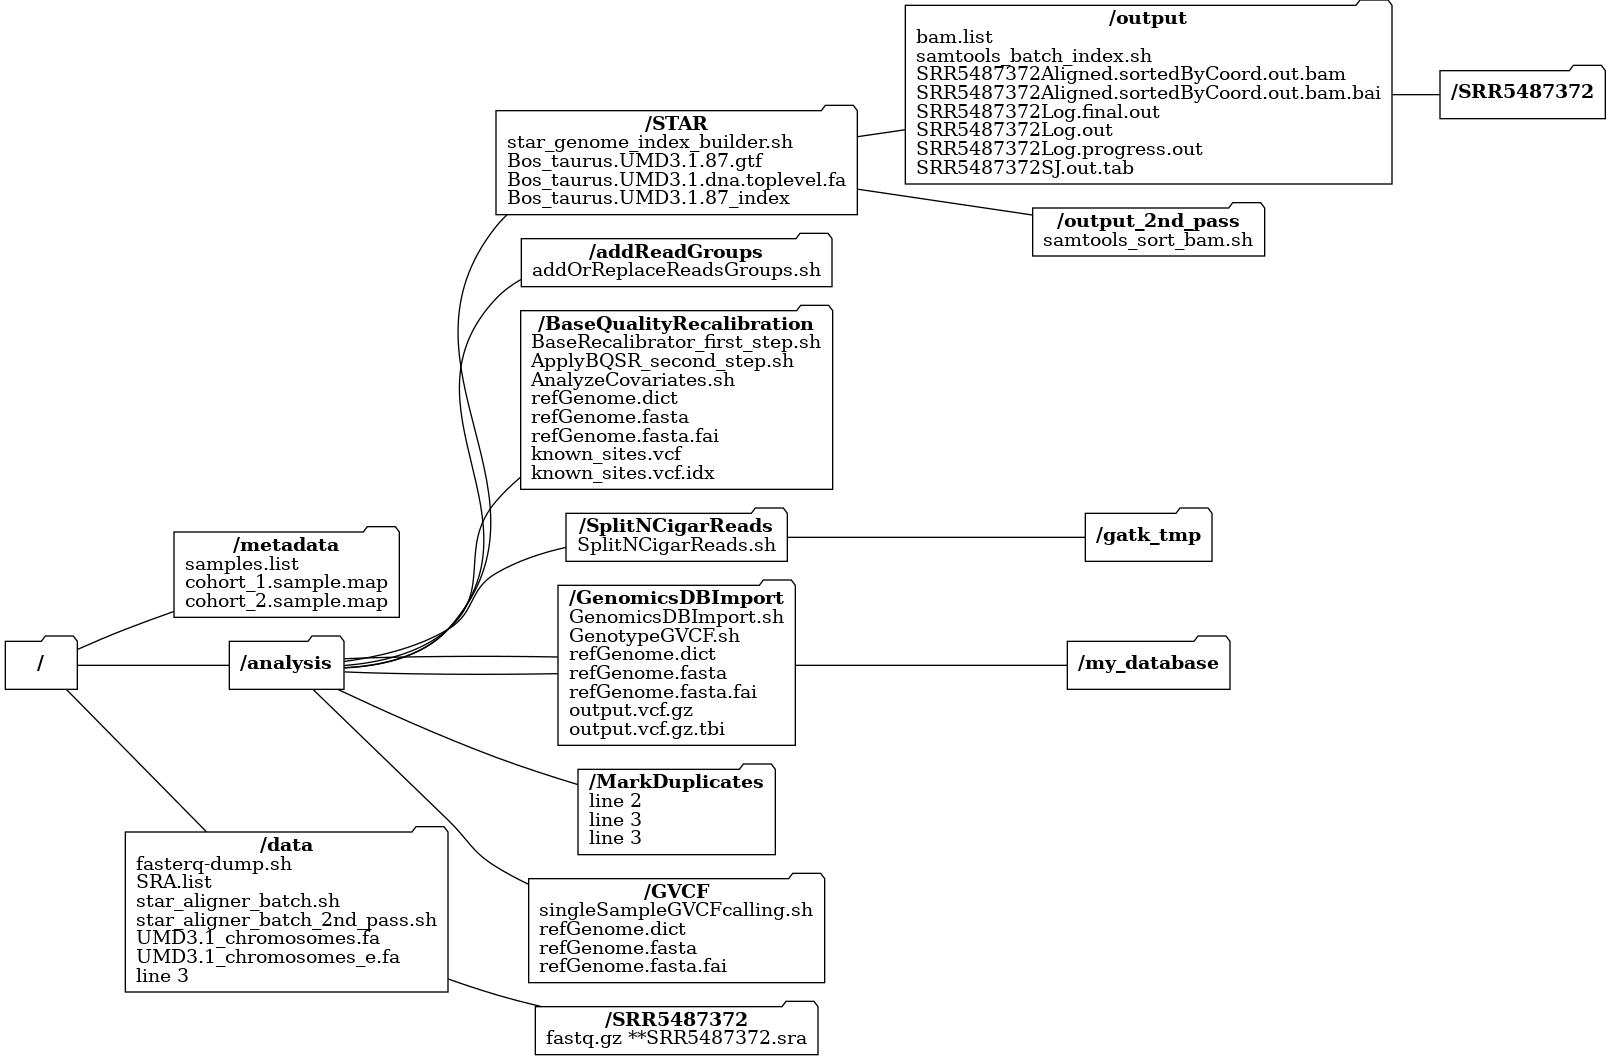
\includegraphics[width=\textwidth]{misc/tree.png}
\caption[caption] {long desc.}

\end{center}
\end{figure}





\subsection{Downloading sequences from NCBI SRA}

In this tutorial, we choose to work with full-length RNAseq datasets derived from macrophage transcriptomes of cows in response to the infection by \textit{Mycobacterium avium ssp. paratuberculosis } (MAP), the etiological agent of paratuberculosis, or Johne’s disease (JD) \cite{Ariel2021}. A representative subset of 24 samples was selected for which the SRA identifiers can be found in the data/SRA.list file.

\begin{verbatim}
SRS2153774
SRS2153779
SRS2153781
...
SRS2153841
SRS2153845
\end{verbatim}


To download these sequences (221 Gb), navigate to the /data directory and download the samples with the prefetch command from the SRAtoolkit:

\begin{verbatim}
prefetch --option-file SRA.list
\end{verbatim}

To extract fastq files from .sra archives, the fasterq-dump command is required. For example, the following command will produce SRR5487396\_R1.fastq.gz and SRR5487396\_R2.fastq.gz:

\begin{verbatim}
fasterq-dump --split-files SRR5487396/SRR5487396.sra
\end{verbatim}

In practice, you will want to extract all downloaded sequence read archives, which are nested in distinct folders. Navigate to the /data folder and use the following qsub command to lauch the faster-qdump commands sequentially:

\begin{verbatim}
qsub -V -S /bin/bash -cwd -j y -pe smp 12 faster-qdump_sequential.sh
\end{verbatim}

where faster-qdump\_sequential.sh is a bash script containing instructions for the SGE workload manager and the code to iterate on downloaded archives and to produce the forward and reverse fastq files;

\begin{verbatim}
#! /bin/bash
#$ -N 'fasterq-dump'
#$ -o ./faster-qdump_log.txt
	
for i in `ls -d SRR*`; do
cd $i
fasterq-dump --split-files $i.sra
cd ..
done
\end{verbatim}


However, executing the latter script would take a lot of times. To take advantage of the parallel computing capacity of compute servers, one may consider launching SGE task array jobs (tasks in parallel). This can be done by using the SGE task array capabilities. Briefly, a single script is run multiple times with different values taken by the single environment variable \$SGE\_TASK\_ID. Using an UNIX trick on a list of samples, each instance of the script can be run on a distinct dataset. Since many bioinformatic tasks used in this tutorial are computationally intensive, most of the scripts presented thereafter will be base on this model. For brevity, we did not include most of the required SGE options (lines beginning with \#\$ within BASH scripts. Therefore, it is important to include them with the qsub command. For example, in this tutorial, launch parallel tasks (with 24 samples) with:
\begin{verbatim}
qsub -V -S /bin/bash -cwd -j y -t 1-24 -pe smp 4 parallel_task.sh \
\end{verbatim}

Otherwise, omit the -t option and increase the number of cores to be used:
\begin{verbatim}
qsub -V -S /bin/bash -cwd -j y -pe smp 12 unparallel_task.sh \
\end{verbatim}


Before lauching the parallel version of fasterq.dump.sh, create a simple list of the 24 SRR* folders present in the /data folder:

\begin{verbatim}
ls -d1 SRR5487???>SRR.list
\end{verbatim}

The SRR.list file should contain the 24 SRR identifiers (without the .sra extension) on separates lines. You are now ready to execute the faster-qdump\_parallel.sh listing:

\begin{verbatim}
#!/bin/bash
#$ -N fasterq-dump
#$ -o ./fasterq-dump.$TASK_ID.log
	
input=$(head -n $SGE_TASK_ID SRR.list | tail -n 1)
	
cd $input
fasterq-dump --split-files $input.sra
cd ..
\end{verbatim}
















\section{Methods}



\subsection{Mapping Reads to Reference (STAR 2-pass)}



\subsubsection{Generating Genome Indexes Files}
The current recommendation of the GATK Per-sample RNAseq  workflow is to perform 2-pass mapping with the STAR aligner \cite{Dobin2013}. STAR genomes are made available for a limited number of genomes by the Gingeras lab. Here we will use the \textit{Bos taurus} UMD3.1.87 annotations file since the UMD 3.1.1/bosTau8 version of the genome was used in \citep{Ariel2021}. The GTF file describes all exons whereas the .dna.toplevel.fa FASTA file contains the corresponding sequences.

\begin{verbatim}
wget http://labshare.cshl.edu/shares/gingeraslab/www-data/dobin/\
STAR/STARgenomes/Old/ENSEMBL/bos_taurus/Bos_taurus.UMD3.1.87.gtf;

wget http://labshare.cshl.edu/shares/gingeraslab/www-data/dobin/\
STAR/STARgenomes/Old/ENSEMBL/bos_taurus/\
Bos_taurus.UMD3.1.dna.toplevel.fa;
\end{verbatim}

To prepare genome index files for STAR, use the genomeGenerate built-in STAR command.
Note that you have to create a directory where STAR could build the index:

\begin{verbatim}
mkdir Bos_taurus.UMD3.1.87_index
\end{verbatim}

Then, build the index with the star\_genome\_index\_builder.sh:
\begin{verbatim}
#! /bin/bash
#$ -N 'STAR_genome_builder'
#$ -o ./star_genome_builder_log.txt
STAR --runThreadN 12 \
--runMode genomeGenerate \
--genomeDir Bos_taurus.UMD3.1.87_index \
--genomeFastaFiles ./Bos_taurus.UMD3.1.dna.toplevel.fa \
--sjdbGTFfile ./Bos_taurus.UMD3.1.87.gtf \
--sjdbOverhang 99
\end{verbatim}



\subsubsection{Aligning RNAseq reads (1st mapping pass)}

At this step, we align our raw FASTQ files with the STAR aligner:

\begin{verbatim}
#!/bin/bash
#$ -N 'STAR_aligner'
#$ -o STAR_aligner_1st_pass.$TASK_ID.log
input=$(head -n $SGE_TASK_ID SRR.list | tail -n 1)
mkdir -p ../analysis/STAR/output/$input
STAR --genomeDir ./Bos_taurus.UMD3.1.87_index \
--runThreadN 12 \
--readFilesIn  ./$input/$input"_1.fastq" ./$input/$input"_2.fastq" \
--outFileNamePrefix ../analysis/STAR/output/$input \
--outSAMtype BAM SortedByCoordinate \
--outSAMunmapped Within \
--outSAMattributes Standard
\end{verbatim}



\subsubsection{Aligning RNAseq reads (2nd mapping pass)}

The 2nd mapping pass is identical to the first alignment except that all splice junctions discovered in the first pass are given as input to the programs, allowing to detect more reads mapping to novel junctions  \cite{Dobin2013}. Simply specify a list of all splice junctions files after the --sjdbFileChrStartEnd argument in the star\_aligner\_2nd\_pass.sh listing:

\begin{verbatim}
#!/bin/bash
#$ -N 'STAR_aligner_2nd_pass'
#$ -o STAR_aligner_2nd_pass.$TASK_ID.log
input=$(head -n $SGE_TASK_ID SRR.list | tail -n 1)
mkdir -p ../analysis/STAR/output_2nd_pass/$input
STAR --genomeDir ./Bos_taurus.UMD3.1.87_index \
--runThreadN 4 \
--readFilesIn  ./$input/$input"_1.fastq" ./$input/$input"_2.fastq" \
--outFileNamePrefix ../analysis/STAR/output_2nd_pass/$input \
--outSAMtype BAM SortedByCoordinate \
--outSAMunmapped Within \
--outSAMattributes Standard \
--outTmpDir ../analysis/STAR/output_2nd_pass/_STARtmp_$SGE_TASK_ID \
--sjdbFileChrStartEnd \
../analysis/STAR/output/SRR5487372SJ.out.tab \
../analysis/STAR/output/SRR5487384SJ.out.tab \
...
../analysis/STAR/output/SRR5487430SJ.out.tab \
../analysis/STAR/output/SRR5487442SJ.out.tab
\end{verbatim}



\subsubsection{Sorting Alignment Files}


Once the RNA sequences are aligned, you will want your BAM files to be indexed and sorted by coordinates. As mentioned earlier, STAR allows the output to be sorted by coordinates. If you have carefully followed this tutorial, there is no need to sort again your BAM files and you can safely ignore the next step and jump to the next subheading. However, if for any reasons, your aligmnents files are not sorted adequately, the sorting by coordinates with the Samtools is as easy as :

\begin{verbatim}
samtools sort file.bam -o file_sorted.bam
\end{verbatim}

In a folder containing unsorted alignments, first prepare a list of bam files to be sorted with:

\begin{verbatim}
ls -1 *.bam > bam.list
\end{verbatim}

Then, we could re-sort our alignments files with the \noindent samtools\_sort\_bam.sh script:

\begin{verbatim}
#!/bin/bash
#$ -V
#$ -N samtools_sort
#$ -o samtools_sort.$TASK_ID.log
input=$(head -n $SGE_TASK_ID bam.list | tail -n 1 | xargs \
basename -s '.bam')
samtools sort $input.bam -o $input"_sorted.bam"
\end{verbatim}

Note that this listing could be used as a template to perform a variety of Samtools subcommands that involve renaming output files.

\subsubsection{Indexing Alignment Files}

BAM files, the binary analog of Sequence Alignment Mapping (SAM) files,  are very efficient bioinformatic files designed to store high-throughput alignment data. Typically, they contain the result of the alignment of millions of sequencing reads against a reference genome and greatly benefit from being indexed by genomic positions for faster random access to the aligned reads at a specific locus \cite{DataSkills}. In practice most programs will not run in the absence of index files. Obviously, BAM files need to be sorted before being indexed. To index all BAM files present in the STAR output\_2nd\_pass folder, first prepare a list of files to be indexed with:

\begin{verbatim}
ls -1 *.bam > bam.list
\end{verbatim}

Then, you can index all alignements in parallel with the following samtools\_batch\_index.sh script:

\begin{verbatim}
#!/bin/bash
#$ -N samtools_index
#$ -o samtools_index.$TASK_ID.log
input=$(head -n $SGE_TASK_ID bam.list | tail -n 1)
samtools index $input
\end{verbatim}





\subsection{Adding Read Groups}

Contrarily to FASTQ files, SAM files have the capacity to handle large amount of metadata. A good practice would be to always include informations about the reference genome and the samples in aligment files. Informations about the processing steps could also be stored. Many programs, such as GATK, automatically add this kind of metadata information when manipulating SAM/BAM files.


Most GATK commands involving BAM files require that read groups have been defined. This step ensure that relevant information about the sequencing process follow each read in downstream processing. In addition, when this step is done appropriately, it allow to mitigate the consequences of artifacts associated with sequencing features in the duplicate marking and base recalibration steps \cite{GATK_ReadGroups}. For example, when samples are multiplexed, it is important to known which reads origin from which library, which were sequenced on which flowcell, etc. The GATK engine requires the presence of several read group fields to run without errors. To learn more about the Read groups as understand by the GATK team and to learn how to derive this information from read names, one should consult this page: \href{https://gatk.broadinstitute.org/hc/en-us/articles/360035890671-Read-groups}{https://gatk.broadinstitute.org/hc/en-us/articles/360035890671-Read-groups}.

Here, we will set the flowcells, sequencing lanes and sample barcodes in the PU (Platform Unit) tag. We will also set the PL (Platform/technology used to produce the read) and LB (DNA preparation library identifier) tags. Note that the ID (Read group identifier) tag is overrided by the PU tag for base recalibration when the latter is defined.

Before running the main script, we will extract the first and fifth columns from our metadata file and place them in separate files, namely RGLB.txt and  RGPU.txt, that will be used to populate the LB and PU read groups fields:

\begin{verbatim}
# Corresponding to the sample name
cut -f 1 -d ',' ../../metadata/metadata.csv | tail -n +2 > RGLB.txt

# Corresponding to the PU tag 
cut -f 5 -d ',' ../../metadata/metadata.csv | tail -n +2 > RGPU.txt
\end{verbatim}

where /metadata/metadata.csv looks like:

\begin{verbatim}
sample,cowID,SRAID,Run,RGPU
A_CTL24,cowA,SRS2153774,SRR5487372,C5NL3ACXX.1.CAGATC
A_MAP24,cowA,SRS2153779,SRR5487376,C5NL3ACXX.1.TGACCA
B_CTL24,cowB,SRS2153781,SRR5487378,C5NL3ACXX.3.TGACCA
B_MAP24,cowB,SRS2153786,SRR5487382,C5NL3ACXX.3.GTGAAA
C_CTL24,cowC,SRS2153787,SRR5487384,C5K8FACXX.3.AGTCAA
C_MAP24,cowC,SRS2153791,SRR5487388,C5K8FACXX.3.GTCCGC
D_CTL24,cowD,SRS2153793,SRR5487390,C5K8FACXX.1.TGACCA
...
K_CTL24,cowK,SRS2153835,SRR5487432,C547FACXX.5.AGTCAA
K_MAP24,cowK,SRS2153839,SRR5487436,C547FACXX.5.GTCCGC
L_CTL24,cowL,SRS2153841,SRR5487438,C547FACXX.7.AGTCAA
L_MAP24,cowL,SRS2153845,SRR5487442,C547FACXX.7.GTCCGC
\end{verbatim}


The RGLB.txt file will therefore hold the library name for each 24 samples (e.g. C\_MAP24, which designates a RNAseq library done on the cowC 24h post-infection with the MAP pathogen). The RGPU.txt store the Platform Unit tag, which is made of three types of informations: the flowcell, the sequencing lane and the barcode identifiers, with the following format: {FLOWCELL\_BARCODE}.{LANE}.{SAMPLE\_BARCODE}. Use the following listing to add read groups to our alignments files:


\begin{verbatim}
#!/bin/bash
#$ -N AddOrReplaceReadGroups
#$ -o logfile.$TASK_ID.log
eval "$(conda shell.bash hook)"
conda activate gatk4
SAMPLES="$HOME/jsb/RNAseq_GATK_JGW/metadata/samples.list"
BAMPATH="$HOME/jsb/RNAseq_GATK_JGW/analysis/STAR/output_2nd_pass"
OUTPUT="$HOME/jsb/RNAseq_GATK_JGW/analysis/addReadGroups"
readarray -t RGLB < ./RGLB.txt
readarray -t RGPU < ./RGPU.txt
input=$(head -n $SGE_TASK_ID $SAMPLES | tail -n 1)
java -jar $PICARD AddOrReplaceReadGroups \
	I=$BAMPATH/$input"Aligned.sortedByCoord.out.bam" \
	O=$OUTPUT/$input".bam" \
	RGLB=${RGLB[$SGE_TASK_ID -1]} \
	RGPL=ILLUMINA \
	RGPU=${RGPU[$SGE_TASK_ID -1]} \
	RGID=${RGPU[$SGE_TASK_ID -1]} \
	RGSM=$input
conda deactivate
\end{verbatim}

Note that the value given by \$SGE\_TASK\_ID -1 was used to fetch the correct values in RGLB and RGPU arrays because Bash arrays are zero-indexed.

After completion of the previous step, we will want to validate that the reads groups have been correctly set. When present, read groups are written in the header of BAM files. Thus, this simple UNIX trick allows one to quickly inspect the read groups associated to a BAM file:

\begin{verbatim}
samtools view -H sample.bam | grep '@RG'	
\end{verbatim}


To see read groups on all our BAM files, use something like:

\begin{verbatim}
for i in `ls *.bam | xargs basename -s '.bam'`;\
do samtools view -H $i.bam | grep '@RG'; done
\end{verbatim}

\begin{small}
\begin{verbatim}
@RG	ID:C5NL3ACXX.1.CAGATC	LB:A_CTL24	PL:ILLUMINA	SM:SRR5487372	PU:C5NL3ACXX.1.CAGATC
@RG	ID:C5NL3ACXX.1.TGACCA	LB:A_MAP24	PL:ILLUMINA	SM:SRR5487376	PU:C5NL3ACXX.1.TGACCA
@RG	ID:C5NL3ACXX.3.TGACCA	LB:B_CTL24	PL:ILLUMINA	SM:SRR5487378	PU:C5NL3ACXX.3.TGACCA
@RG	ID:C5NL3ACXX.3.GTGAAA	LB:B_MAP24	PL:ILLUMINA	SM:SRR5487382	PU:C5NL3ACXX.3.GTGAAA
\end{verbatim}
\end{small}






\subsection{Marking Duplicates Reads}


Duplicate reads can arise from PCR duplication artifacts that take place during the library construction or from reading errors that occur during the sequencing process (optical duplicates). Regardless of their origin, these reads need at least to be identified in alignment files. The MarkDuplicate program from the Picard tools have many other options to deal with these issues. For example, the program offers the possibility to completely remove the duplicate reads and to make the distinction between the optical and PCR duplicates. In the MarkDuplicates.sh listing we simply identify the duplicate reads in our BAM files before proceeding to the next step:

\begin{verbatim}
#!/bin/bash
#$ -N MarkDuplicates
#$ -o logfile.$TASK_ID.log
SAMPLES="$HOME/jsb/RNAseq_GATK_JGW/metadata/samples.list"
BAMPATH="$HOME/jsb/RNAseq_GATK_JGW/analysis/addReadGroups"
OUTPUT="$HOME/jsb/RNAseq_GATK_JGW/analysis/MarkDuplicates"
input=$(head -n $SGE_TASK_ID $SAMPLES | tail -n 1)
java -jar $PICARD MarkDuplicates \
	I=$BAMPATH/$input".bam" \
	O=$OUTPUT/$input"_marked_duplicates.bam" \
	M=$OUTPUT/$input"_marked_dup_metrics.txt"
\end{verbatim}

\subsection{Splitting RNAseq reads}

With the alignment of RNAseq reads, the SplitNCigarReads step, (formerly called SplitNTrim step in previous versions of GATK workflows), is highly specific to RNAseq analysis. During this process, reads that span splice junctions (for example reads that align over distinct exons) are split in smaller reads and map to the right location in new alignments files.

\subsubsection{Preparing Reference Genome Files}

Until now, we have work with STAR reference genome which barely contains sequences that are transcribed in RNA. In contrast, the GATK SplitNCigarReads command requires a complete reference sequence as input. At this point, one should be advised to download the same version of the refence genome that was used to prepare the STAR genome.

Here we use the Bovine Genome Database (\href{https://bovinegenome.elsiklab.missouri.edu/}{https://bovinegenome.elsiklab.missouri.edu/}) to get the UMD3.1 assembly.

\begin{verbatim}
wget http://128.206.12.216/drupal/sites/bovinegenome.org/\
files/data/umd3.1/UMD3.1_chromosomes.fa.gz
gunzip UMD3.1_chromosomes.fa.gz
\end{verbatim}


The bovine genome database also contains several annotations files for the UMD3.1 assembly. We will use the Ensembl annotation file of protein and non-protein-coding genes when visualizing alignments with genome browsers at the end of this tutorial.

\begin{verbatim}
wget http://128.206.12.216/drupal/sites/bovinegenome.org/\
files/data/umd3.1/Ensembl79_UMD3.1_genes.gff3.gz
gunzip Ensembl79_UMD3.1_genes.gff3.gz
\end{verbatim}


It is crucial that entries in the reference genome match the corresponding ones in the STAR genome. If you inspect the FASTA headers of the UMD3.1\_chromosomes.fa, you will notice that each entry contains many fields (e.g. gnl , UMD3.1 Accession numbers):

\begin{verbatim}
grep ">" UMD3.1_chromosomes.fa
output:
>gnl|UMD3.1|GK000010.2 Chromosome 10 AC_000167.1
>gnl|UMD3.1|GK000011.2 Chromosome 11 AC_000168.1
>gnl|UMD3.1|GK000012.2 Chromosome 12 AC_000169.1
...
>gnl|UMD3.1|GK000009.2 Chromosome 9 AC_000166.1
>gnl|UMD3.1|AY526085.1 Chromosome MT NC_006853.1
>gnl|UMD3.1|GK000030.2 Chromosome X AC_000187.1
>gnl|UMD3.1|GJ057137.1 GPS_000341577.1 NW_003097882.1
>gnl|UMD3.1|GJ057138.1 GPS_000341578.1 NW_003097883.1
...
\end{verbatim}

In contrast, the chromosomes entries in the STAR genome are quite different:

\begin{verbatim}
cat Bos_taurus.UMD3.1.87_index/chrName.txt | head -n 32
output:
1
10
11
...
9
MT
X
GJ058422.1
\end{verbatim}

Therefore, the chromosome identifiers found in the \textit{Bos taurus} UMD3.1 genome need to be changed to match their counterparts in the STAR genome. This could be achieved with UNIX SED:

\begin{verbatim}
sed -r s'/^>.+Chromosome\s+(\S+)\s+.+/>\1/' UMD3.1_chromosomes.fa \
> temp1.fa
grep ">" temp1.fa | head -n 40

# Handle unassigned scaffolds (accessions that begin with "GJ").
sed -r s'/^>gnl\|UMD3\.1\|(\S+)+\s+.+/>\1/' temp1.fa > temp2.fa
grep ">" temp2.fa | tail -n +30 | head -n 10
mv temp2.fa refGenome.fasta
rm temp1.fa
\end{verbatim}

Note that we have rename the edited UMD3.1\_chromosome assembly file by refGenome.fasta

Along with the reference genome, many GATK tools will need a dictionary file ending in .dict and an index file ending in .fai.(\href{https://gatk.broadinstitute.org/hc/en-us/articles/360035531652-FASTA-Reference-genome-format}{ https://gatk.broadinstitute.org/hc/en-us/articles/360035531652-FASTA-Reference-genome-format}). It is mandatory that these files share the same basename as the reference genome. You can prepare the index with:

\begin{verbatim}
samtools faidx refGenome.fasta
\end{verbatim}

On the other hand, use the GATK CreateSequenceDictionary tool to create the required .dict file:

\begin{verbatim}
gatk CreateSequenceDictionary -R refGenome.fasta
\end{verbatim}




\subsubsection{Running SplitNCigarReads}

Having prepared the reference genome, we are ready to lauch the SplitNCigarRead step:

\begin{verbatim}
#!/bin/bash
#$ -N SplitNCigarReads
#$ -o SplitNCigarReads.$TASK_ID.log
eval "$(conda shell.bash hook)"
conda activate gatk4
SAMPLES="$HOME/jsb/RNAseq_GATK_JGW//metadata/samples.list"
BAMPATH="$HOME/jsb/RNAseq_GATK_JGW/analysis/MarkDuplicates"
OUTPUT="$HOME/jsb/RNAseq_GATK_JGW/analysis/SplitNCigarReads"
input=$(head -n $SGE_TASK_ID $SAMPLES | tail -n 1)
gatk SplitNCigarReads \
	-R refGenome.fasta \
	-I $BAMPATH/$input"_marked_duplicates.bam" \
	-O $OUTPUT/$input"_SplitNCigarReads.bam" \
	--tmp-dir $OUTPUT/gatk_tmp
conda deactivate
\end{verbatim}



\subsection{Performing Base Quality Score Recalibration}

Base Quality Score Recalibration (BQSR) is an optional, but highly recommended step, that is part of DNAseq and RNAseq GATK best practices workflows. This complex procedure, which involves binning and machine learning consist of re-evaluating all base quality scores assigned by sequencing machines which are prone to systematic technical errors \cite{GATK_BaseQuality}. Several features are taken into account, notably the reported quality score, the position within the read and the sequence context. This procedure lead to more accurate base calls, a situation that improve the accuracy of variant calling overall. More details about how the model is build and how new quality scores are computed can be found at \href{https://gatk.broadinstitute.org/hc/en-us/articles/360035890531-Base-Quality-Score-Recalibration-BQSR-}{https://gatk.broadinstitute.org/hc/en-us/articles/360035890531-Base-Quality-Score-Recalibration-BQSR-}.

\subsubsection{Using BaseRecalibrator}

In the first key step  a model of covariation is build with two components: the alignement given as input (BAM files) and a set of known variants (VCF file). The BaseRecalibrator will then produce a recalibration file which is used in the second key step of the procedure. To perform this task one would need a source of reliable variants in the investigated genome. With human data and other common model organisms, it would be easy to find such sources of variants, thanks to the existence of variation databases. Here we use a single VCF file containing the results of the BovineSNP50 genotyping BeadChip to train the model, but you can feed the model with several VCF files.

Before running the BaseRecalibrator command, index the SNP50 VCF file with:

\begin{verbatim}
gatk IndexFeatureFile -I snp50.vcf.gz
\end{verbatim}


The BaseRecalibrator\_first\_step.sh listing:
\begin{verbatim}
#!/bin/bash
#$ -N BaseRecalibrator
#$ -o BaseQualityRecalibration_$TASK_ID.log
eval "$(conda shell.bash hook)"
conda activate gatk4
SAMPLES="$HOME/jsb/RNAseq_GATK_JGW/metadata/samples.list"
BAMPATH="$HOME/jsb/RNAseq_GATK_JGW/analysis/SplitNCigarReads"
OUTPUT="$HOME/jsb/RNAseq_GATK_JGW/analysis/BaseQualityRecalibration"
input=$(head -n $SGE_TASK_ID $SAMPLES | tail -n 1)
gatk BaseRecalibrator \
	-R ../SplitNCigarReads/refGenome.fasta \
	-I $BAMPATH/$input"_SplitNCigarReads.bam" \
	--known-sites ./snp50.vcf.gz \
	-O $OUTPUT/$input"_recal_data.table"
conda deactivate
\end{verbatim}





\subsubsection{Using ApplyBQSR to Adjust the Scores}

In the second step of the BaseQuality recalibration process, the GATK ApplyBQSR command assigns new scores to each base based on the model produced in the first step and produces new BAM files that reflet these changes. Here the ApplyBQSR\_second\_step.sh listing:

\begin{verbatim}
#!/bin/bash
#$ -N ApplyBQSR
#$ -o ApplyBQSR_$TASK_ID.log
eval "$(conda shell.bash hook)"
conda activate gatk4
SAMPLES="$HOME/jsb/RNAseq_GATK_JGW/metadata/samples.list"
BAMPATH="$HOME/jsb/RNAseq_GATK_JGW/analysis/SplitNCigarReads"
OUTPUT="$HOME/jsb/RNAseq_GATK_JGW/analysis/BaseQualityRecalibration"
echo $SAMPLES
input=$(head -n $SGE_TASK_ID $SAMPLES | tail -n 1)
gatk ApplyBQSR \
	-R ../SplitNCigarReads/refGenome.fasta \
	-I $BAMPATH/$input"_SplitNCigarReads.bam" \
	--bqsr-recal-file $OUTPUT/$input"_recal_data.table" \
	-O $OUTPUT/$input"_recal.bam"
conda deactivate
\end{verbatim}

\subsubsection{Comparing pre- and post-recalibration metrics}

To visualize the effect of the procedure, one can build a seconde model and generate plots with data before and after recalibration \cite{GATK_BaseQuality}. The GATK command AnalyzeCovariates was created for that purpose as in the following example:

\begin{verbatim}
gatk AnalyzeCovariates \
-before recal1.table \
-after recal2.table \
-plots AnalyzeCovariates.pdf
\end{verbatim}

The Base recalibration being the final step in the data cleanup part of the workflow present here (figure 1), we are now ready for discovering variants from our analysis-ready RNAseq reads with the joint genoyping approach.

\subsection{Joint Genotyping Variant Calling}

\subsubsection{Calling Variants Per-sample (GVCF mode)}

In this step, the GATK HaplotypeCaller engine identifies candidate variation sites and record them in GVCF files. This is why this step has been called "GVCF workflow". GVCF files act as intermediate between analysis ready reads (BAM files) and the final joint analysis of multiple samples \cite{GATK_jointCalling_1}. Such intermediate files facilitate the incremental discovery of variants and should be kept since they can be reused in novel rounds of joint genotyping analysis. Our listing to produce GVCF files for each sample reads as follow:

\begin{verbatim}
#!/bin/bash
#$ -N GVCF
#$ -o singleSampleCallingGVCF_$TASK_ID.log
eval "$(conda shell.bash hook)"
conda activate gatk4
SAMPLES="$HOME/jsb/RNAseq_GATK_JGW/metadata/samples.list"
BAMPATH="$HOME/jsb/RNAseq_GATK_JGW/analysis/BaseQualityRecalibration"
OUTPUT="$HOME/jsb/RNAseq_GATK_JGW/analysis/GVCF"
echo $SAMPLES
input=$(head -n $SGE_TASK_ID $SAMPLES | tail -n 1)
gatk --java-options "-Xmx4g" HaplotypeCaller \
	 --dont-use-soft-clipped-bases true \
	 -R ../SplitNCigarReads/refGenome.fasta \
	 -I $BAMPATH/$input"_recal.bam" \
	 -O $OUTPUT/$input".g.vcf.gz" \
	 -ERC GVCF
conda deactivate
\end{verbatim}



\subsubsection{Merging of GCVF files}

Merging of GCVF files has been revised recently by GATK experts by the addition of the novel GenomicsDBImport command. It resembles the former CombineGVCFs command, but promises better performances for parsing of VCF files and computing values stored in the VCF INFO fields (\href{https://gatk.broadinstitute.org/hc/en-us/articles/360036883491-GenomicsDBImport}{https://gatk.broadinstitute.org/hc/en-us/articles/360036883491-GenomicsDBImport}). Interestingly, under the hood, this command make use of a novel data managament system called  TileDB which is particluarly useful for representing huge sparse 2D arrays such as the genomic data found in VCF files \cite{Papadopoulos2016}. 


The command requires a map files that list file paths of all GVCF files to be included in the resulting database. The -L option specifies the range of genomic intervals on which the command operate and may be used several times. Here to save time, we will call variants solely on bovine chromosomes 4 and 11:

\begin{verbatim}
#!/bin/bash
#$ -N GenomicsDBImport
#$ -o GenomicsDBImport.log
eval "$(conda shell.bash hook)"
conda activate gatk4
SAMPLES="$HOME/jsb/RNAseq_GATK_JGW/metadata"
OUTPUT="$HOME/jsb/RNAseq_GATK_JGW/analysis/GenomicsDBImport"
gatk --java-options "-Xmx4g -Xms4g" \
	GenomicsDBImport \
	--genomicsdb-workspace-path $OUTPUT/"my_database" \
	-L 4 \
	-L 11 \
	--sample-name-map $SAMPLES/"cohort_1.sample_map" \
	--tmp-dir $OUTPUT/tmp \
	--reader-threads 5
conda deactivate
\end{verbatim}


\subsubsection{Joint Genotyping}

The final step in this variant calling workflow is performed with the GATK GenotypeGVCFs command (  \href{https://gatk.broadinstitute.org/hc/en-us/articles/360037057852-GenotypeGVCFs}{https://gatk.broadinstitute.org/hc/en-us/articles/360037057852-GenotypeGVCFs}). During this operation, all samples for which variants have been pre-called with HaplotypeCaller are jointly genotyped. This step could be rerun when new samples are available, allowing the so-called incremental discovery of variants.


The command take as argument a GenomicsDB workspace created by GenomicsDBImport, which can be seen as a sophisticated database that facilitate the parsing of the genomic data present in GVCF files. Alternatively, a single multi-sample GCVF file produced by CombineGVCFs can also be given as input.

\begin{verbatim}
#!/bin/bash
#$ -N GenotypeGVCF
#$ -o GenotypeGVCF.log
eval "$(conda shell.bash hook)"
conda activate gatk4
gatk --java-options "-Xmx4g" GenotypeGVCFs \
	-R ../SplitNCigarReads/refGenome.fasta \
	-V gendb://my_database \
	-O output.vcf.gz
conda deactivate
\end{verbatim}

\subsection{Querying VCF files}


As mentionned earlier, BCFtools are optimized by design, to query and manipulate VCF files. Therefore, it is worth the pain to familiarize with these tools rather than using the plain VCF files with UNIX tricks. In addition, since BCFtools work well with compressed files it would be a waste of time to compress or extract VCF files not to mention the risk of corrupting or erasing a VCF file. Because one can easily erase a file by mistake when attempting to redirect the result of a command, it is a good practice to keep a copy of the primary VCF output file (output.vcf.gz) in a safe place.

That said, the BCFtools command are highly versatile and can be used in several circumstances ranging from performing simples queries to applying complex filters. Here, we will start by getting a list of the 10 samples present in our VCF file:

\begin{verbatim}
bcftools query -l output.vcf.gz
\end{verbatim}

Remember that we used a subset of 10 samples with the GenomicsDBImport command to highlight the incremental discovery of variants that origin from distinct cohorts of samples.


To get useful metrics, like the sequencing depth or the ratio of transitions and transversions use the built-in stats command:
\begin{verbatim}
bcftools stats output.vcf.gz  > stats.txt
\end{verbatim}

To quickly see the numbers of variants that fall in each category:
\begin{verbatim}
bcftools stats output.vcf.gz | grep -E "^SN"
\end{verbatim}

Again, one should keep in mind that we have import only import chromosomes 4 and 11 in the genomic database, a situation that reduce the number of variants reported:

\begin{verbatim}
output:
SN	0	number of samples:	10
SN	0	number of records:	147755
SN	0	number of no-ALTs:	0
SN	0	number of SNPs:	128421
SN	0	number of MNPs:	0
SN	0	number of indels:	19534
SN	0	number of others:	0
SN	0	number of multiallelic sites:	1520
SN	0	number of multiallelic SNP sites:	89
\end{verbatim}


To mask the VCF header and see selected variants in a specific regions use the BCFtools view subcommand:
\begin{verbatim}
bcftools view -H -r 11:21401262-21402262 -s SRR5487372,SRR5487376,\
SRR5487378 output.vcf.gz
\end{verbatim}



This 1000 bp region contains the rs43668743 that has been shown to be highly associated to susceptibility to bovine paratuberculosis \cite{Ariel2021}.

The BCFtools query subcommand make possible to fetch some VCF columns and format them to the desired output format. Here we will highlight chromosome numbers, positions, overall quality scores, overall read depths and genotypes:

\begin{verbatim}
bcftools query -r 11:21401262-21402262 -s SRR5487372,SRR5487376,\
SRR5487378 -f 'chr%CHROM pos:%POS Q:%QUAL DP=%INFO/DP GT=[ %GT]\n' \
output.vcf.gz
output:
chr11 pos:21401262 Q:304.11 DP=25 GT= 0/1 0/0 1/1
chr11 pos:21401911 Q:152.97 DP=13 GT= 0/0 0/0 ./.
\end{verbatim}



\subsection{Filtering variants}

Contrarily to DNAseq workflows where sophisticated methods for filtering variants are available (e.g. VQSR and CNNScoreVariants), the current recommandation for RNAseq is to use hard filters as described in the canonical RNAseq Best practice RNAseq short variant discovery workflow \cite{GATK_RNAseq_variant_discovery}. The GATK and Picard tools have several commands to filter variants although the BCFtools filter and view commands can also be used. To perform hard filter, one could use the GATK VariantFiltration command  (\href{https://gatk.broadinstitute.org/hc/en-us/articles/360037269391-VariantFiltration}{https://gatk.broadinstitute.org/hc/en-us/articles/360037269391-VariantFiltration}) which is designed to filter variants on the basis of annotations present in INFO or FORMAT VCF fields.

Naturally, the extend of filtration steps that could be done depends on the nature of the downstream analysis that will be performed. Filtering variants is an active aera of research and the reader is invite to consult the GATK Best practices workflows documentation to be aware of all the novelties.

Among the numerous filtering steps that could be done, the first presented here is specific to RNAseq data. It consist of filtering out clusters of at least 3 SNPs that are within a window of 35 bases between them. Note that the following commands can be done interactively in the gatk4 environment. 


\begin{verbatim}
gatk VariantFiltration \
-R refGenome.fasta \
-V output.vcf.gz \
-O filtered.vcf.gz \
--cluster-window-size 35 \
--cluster-size 3
\end{verbatim}

Notice that the GATK command write the strings 'PASS' or 'SnpCluster' in the FILTER field (rather than the dot that was present in the original output VCF file) and add the following lines to the VCF header:

\begin{verbatim}
##FILTER=<ID=SnpCluster,Description="SNPs found in clusters">
##FILTER=<ID=PASS,Description="All filters passed">
\end{verbatim}


Thus, to actually get rid off these variants, we can use the BCFtools view command with the --apply-filter option:
\begin{verbatim}
bcftools view --apply-filters .,PASS filtered.vcf.gz | bgzip -c \
> filtered_2.vcf.gz
\end{verbatim}


Note how the BCFtools are fully integrated with other UNIX commands. Here the filtered VCF files is given to the HSTlib bgzip program that compress it before that the UNIX file redirection operator write the result to a new file. You can validate that SNP clusters do not appear in the output file with:


\begin{verbatim}
bcftools view filtered_2.vcf.gz | grep SnpCluster
\end{verbatim}

In DNA-seq, the generic current recommendation is to filter out variants based on Fisher Strand values (FS > 60.0) and Quality by depth values (QD < 2.0).

At first, we could be interested to know how many variants will be excluded with FS > 60.0:

\begin{verbatim}
bcftools filter -i 'FS > 60' filtered_2.vcf.gz | bcftools view -H \
| wc -l
2610
\end{verbatim}

and how many variants will be excluded with QD < 2.0:

\begin{verbatim}
bcftools filter -i 'QD < 2.0' filtered_2.vcf.gz | bcftools view -H \
| wc -l
15089
\end{verbatim}


To correctly translate the previous recommendation and combine the two criterions, one would be advised to use the logical '||' operator (OR) (rather than '\&\&' (AND)) because one will want to throw out any variants with 'FS > 60' or 'QD < 2.0'. Therefore, to know how many variants will be excluded use: 

\begin{verbatim}
bcftools filter -i 'FS > 60 || QD < 2.0' filtered_2.vcf.gz \
| bcftools view -H | wc -l
17273
\end{verbatim}

To actually remove these variants, simply use the -e option (--exclude) and create a new file:

\begin{verbatim}
bcftools filter -e 'FS > 60 || QD < 2.0' filtered_2.vcf.gz \
| bgzip -c > filtered_3.vcf.gz
\end{verbatim}

Another reasonable hard filtering that can be done would be to exclude calls with poor quality or low read depth:

\begin{verbatim}
bcftools filter -e "QUAL < 20.0 || INFO/DP < 10" filtered_3.vcf.gz \
> filtered_4.vcf.gz
\end{verbatim}

A very intersting ressource to adequately applying other hard filters can be found at \href{https://gatk.broadinstitute.org/hc/en-us/articles/360035890471-Hard-filtering-germline-short-variants}{https://gatk.broadinstitute.org/hc/en-us/articles/360035890471-Hard-filtering-germline-short-variants}.





\subsection{Examining and Visualizing Alignment files}

Visualize alignments allow one to see the distribution of reads on the complete reference genome. This step is helpful to detect potential misaligned regions or other artifacts. Tablet (\href{https://ics.hutton.ac.uk/tablet/download-tablet/}{https://ics.hutton.ac.uk/tablet/download-tablet/}) and the Integrated Genome viewer (\href{https://software.broadinstitute.org/software/igv/}{https://software.broadinstitute.org/software/igv/}) are good choices for such tasks.


\subsubsection{Tweaking the GFF3 file}



If you are interested to add a genome track representing annotated features, the Ensembl UMD 3.1 GFF3 file mentionned in subsection 3.4 is your best option. However, as previously, chromosome names in this file differ from those present in the STAR genome and consequently from those present in our alignment files. With the command below, one can see the identifiers present in the GFF3 file as well as the number of features associated with them :

\begin{verbatim}
cat Ensembl79_UMD3.1_genes.gff3 | cut -f 1 | uniq -cd
\end{verbatim}


\noindent output:
\begin{verbatim}
21287 GK000001.2
18819 GK000030.2
26235 GK000002.2
29793 GK000003.2
...
3 GJ060027.1
3 GJ058256.1
\end{verbatim}

We therefore need to replace the pattern used for the chromosome IDs (GK + 0000 + chromosome number) by solely the chromosome number. This could be done easily with sed:

\begin{verbatim}
sed -r s'/^GK[0]+([0-9]+).2/\1/'g Ensembl79_UMD3.1_genes.gff3 \
> Ensembl79_UMD3.1_genes_e.gff3
\end{verbatim}

As always, the edited file should be inspected to ensure that the desired changes have been done properly.


\subsubsection{Visualizing reads from sample SRR5487372 at a specific locus}

\begin{figure}
\begin{center}

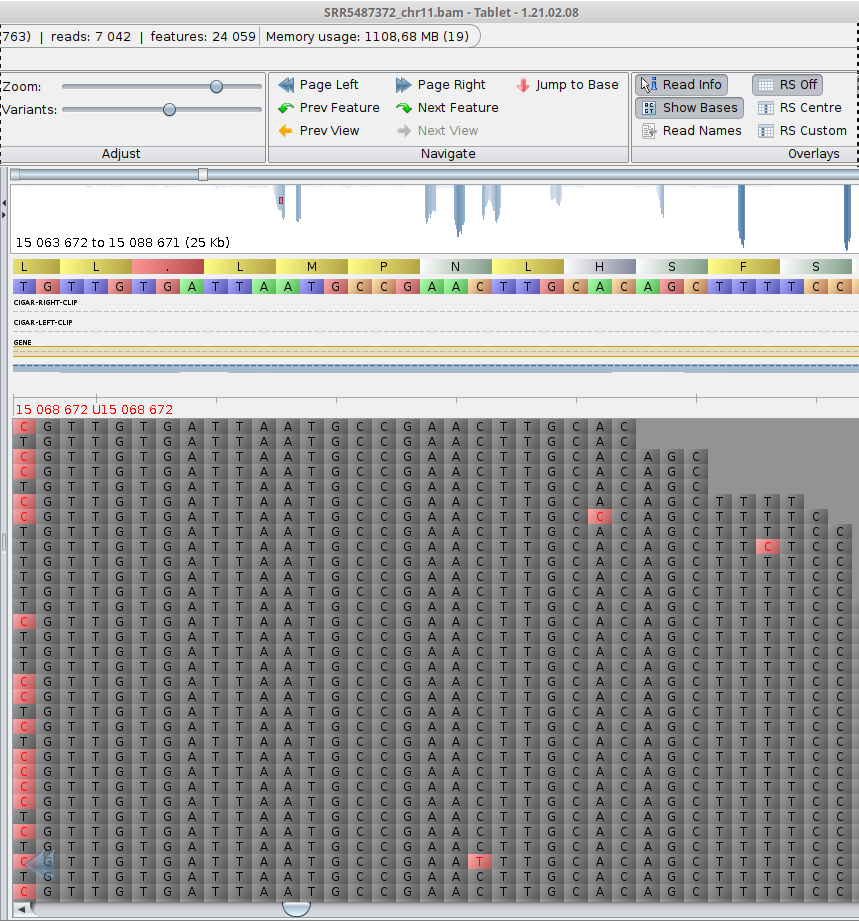
\includegraphics[width=1\textwidth]{misc/SRR5487372_chr11_15068672T_C.png}
\caption[caption] {long desc.}

\end{center}
\end{figure}




We will firstly extract the desired region to be investigated with the Samtools view command:

\begin{verbatim}
samtools view -h -b SRR5487372_recal.bam 1:21000000-22000000 > \
SRR5487372_chr11_region.bam
\end{verbatim}


Then, index this small BAM file and load it in one of the two abovementioned genome browsers. Additionnaly, you will need to provide the appropriate reference genome (refGenome.fasta) as well as its index (refGenome.fasta.fai). You will also want the Ensembl79\_UMD3.1\_genes\_e.gff3 file to be loaded in an annotation track. Navigating to coordinates 21,401,262 you should be able to see why the GATK engine has called an heterozygous call at this locus (figure 3). In the upper panel we can also see that many more reads accumulate in exonic regions of the \textit{SOS} gene.









\bibliographystyle{unsrtnat}
\bibliography{bibliography/RNAseq_VC}





\end{document}
